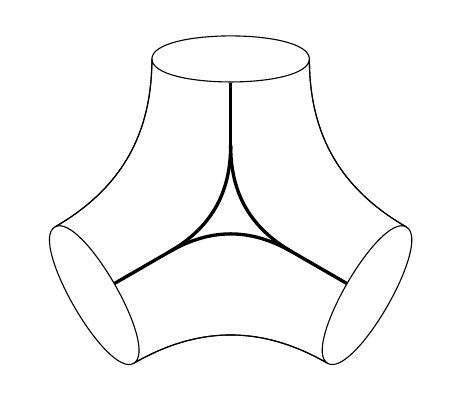
\begin{tikzpicture}[scale=1, very thick]

\coordinate (A1) at (-1, 2);
\coordinate (B1) at (1, 2);

\begin{scope} [rotate=120]
    \coordinate (A2) at (-1, 2);
    \coordinate (B2) at (1, 2);
\end{scope}

\begin{scope} [rotate=240]
    \coordinate (A3) at (-1, 2);
    \coordinate (B3) at (1, 2);
\end{scope}

\draw [thin, fill=none] (A1) 
 to [out=270, in=30] (B2) to [out=30, in=30, looseness=0.5] (A2)
 to [out=30, in=150] (B3) to [out=150, in=150, looseness=0.5] (A3) 
 to [out=150, in=270] (B1) to [out=270, in=270, looseness=0.5] (A1);
\draw [thin] (A1) to [out=90, in=90, looseness=0.5] (B1);
\draw [thin] (A2) to [out=210, in=210, looseness=0.5] (B2);
\draw [thin] (A3) to [out=330, in=330, looseness=0.5] (B3);

\draw [thin] (A1) to [out=270, in=30] (B2);
\draw [thin] (A2) to [out=30, in=150] (B3);
\draw [thin] (A3) to [out=150, in=270] (B1);

\draw (90:1.7) to (90:0.9);
\draw (210:1.7) to (210:0.9);
\draw (330:1.7) to (330:0.9);
\draw (90:0.9) to [out=270, in=30] (210:0.9);
\draw (210:0.9) to [out=30, in=150] (330:0.9);
\draw (330:0.9) to [out=150, in=270] (90:0.9);

\end{tikzpicture}